\newpage
\section*{Dùng công cụ Excel, SPSS, Python và R tính toán}

\section{Thực hiện Logistic Regression bằng Excel}

Bài toán sử dụng mô hình hồi quy logistic nhị phân để dự đoán xác suất tử vong của bệnh nhân dựa trên chỉ số PROCALCITONIN.

\subsection{Cơ sở lý thuyết}

Trong hồi quy logistic, xác suất xảy ra biến cố (tử vong) được mô hình hóa như sau:

\[
p = P(Y=1|X) = \frac{1}{1 + e^{-z}}
\]

Trong đó:

\[
z = \beta_0 + \beta_1 X
\]

Ngoài ra, ta có dạng logit:

\[
\log\left(\frac{p}{1-p}\right) = \beta_0 + \beta_1 X
\]

Hàm hợp lý (Likelihood) của mô hình:

\[
L(\beta) = \prod_{i=1}^{n} p_i^{y_i} (1-p_i)^{1-y_i}
\]

Log-Likelihood:

\[
\ell(\beta) = \sum_{i=1}^{n} \left[ y_i \ln(p_i) + (1-y_i)\ln(1-p_i) \right]
\]

Mục tiêu là:

\[
\max_{\beta_0, \beta_1} \ell(\beta)
\]

\subsection{Các bước thực hiện}

\begin{enumerate}

\item Nhập dữ liệu

Nhập dữ liệu gồm các biến:
\begin{itemize}
\item ID: mã bệnh nhân
\item PROCALCITONIN (X)
\item DEATH (Y)
\end{itemize}

\begin{figure}[!htp]
    \centering
    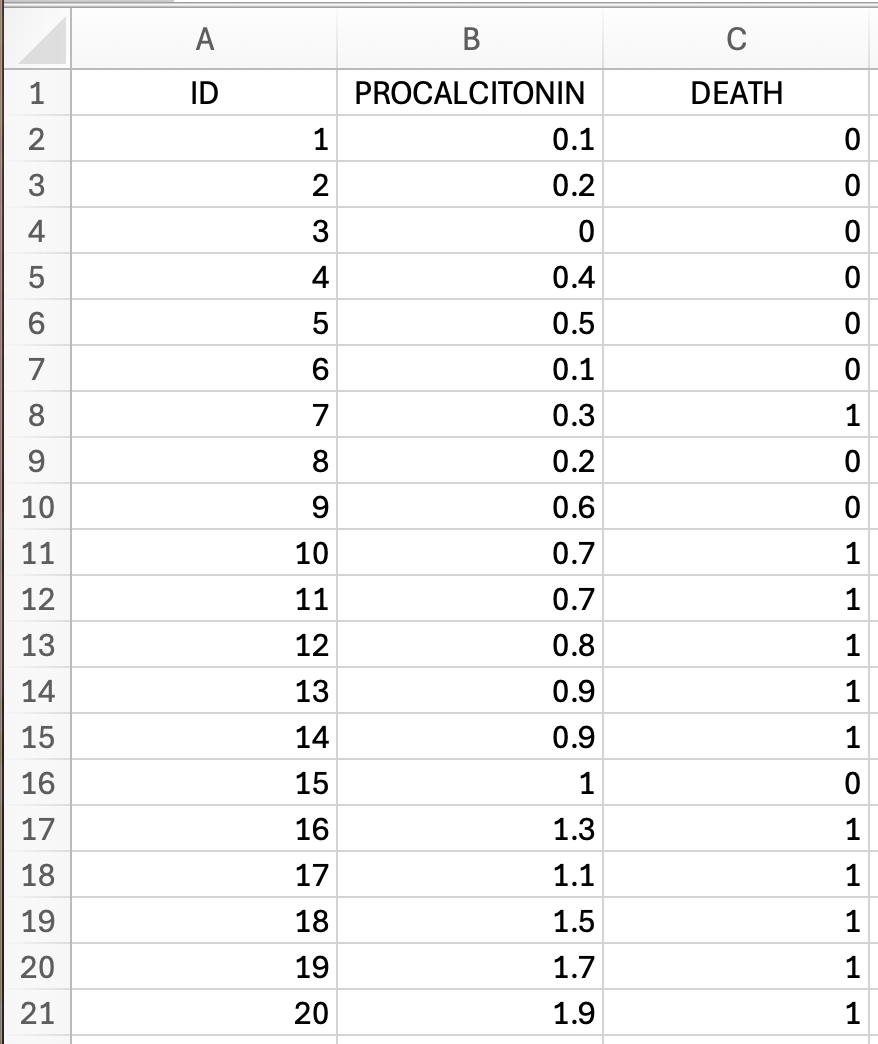
\includegraphics[width=0.6\textwidth]{LAB04/pics/Excel_data.png}
    \caption{Bảng dữ liệu đầu vào trong Excel}
    \label{fig:data}
\end{figure}

\item Tính giá trị tuyến tính $z$

\[
z_i = \beta_0 + \beta_1 X_i
\]

\item Tính xác suất bằng hàm sigmoid

\[
p_i = \frac{1}{1 + e^{-z_i}}
\]

\item Tính Log-Likelihood cho từng quan sát

\[
LL_i = y_i \ln(p_i) + (1-y_i)\ln(1-p_i)
\]

\item Tính tổng Log-Likelihood

\[
\ell(\beta) = \sum_{i=1}^{n} LL_i
\]

\begin{figure}[!htp]
    \centering
    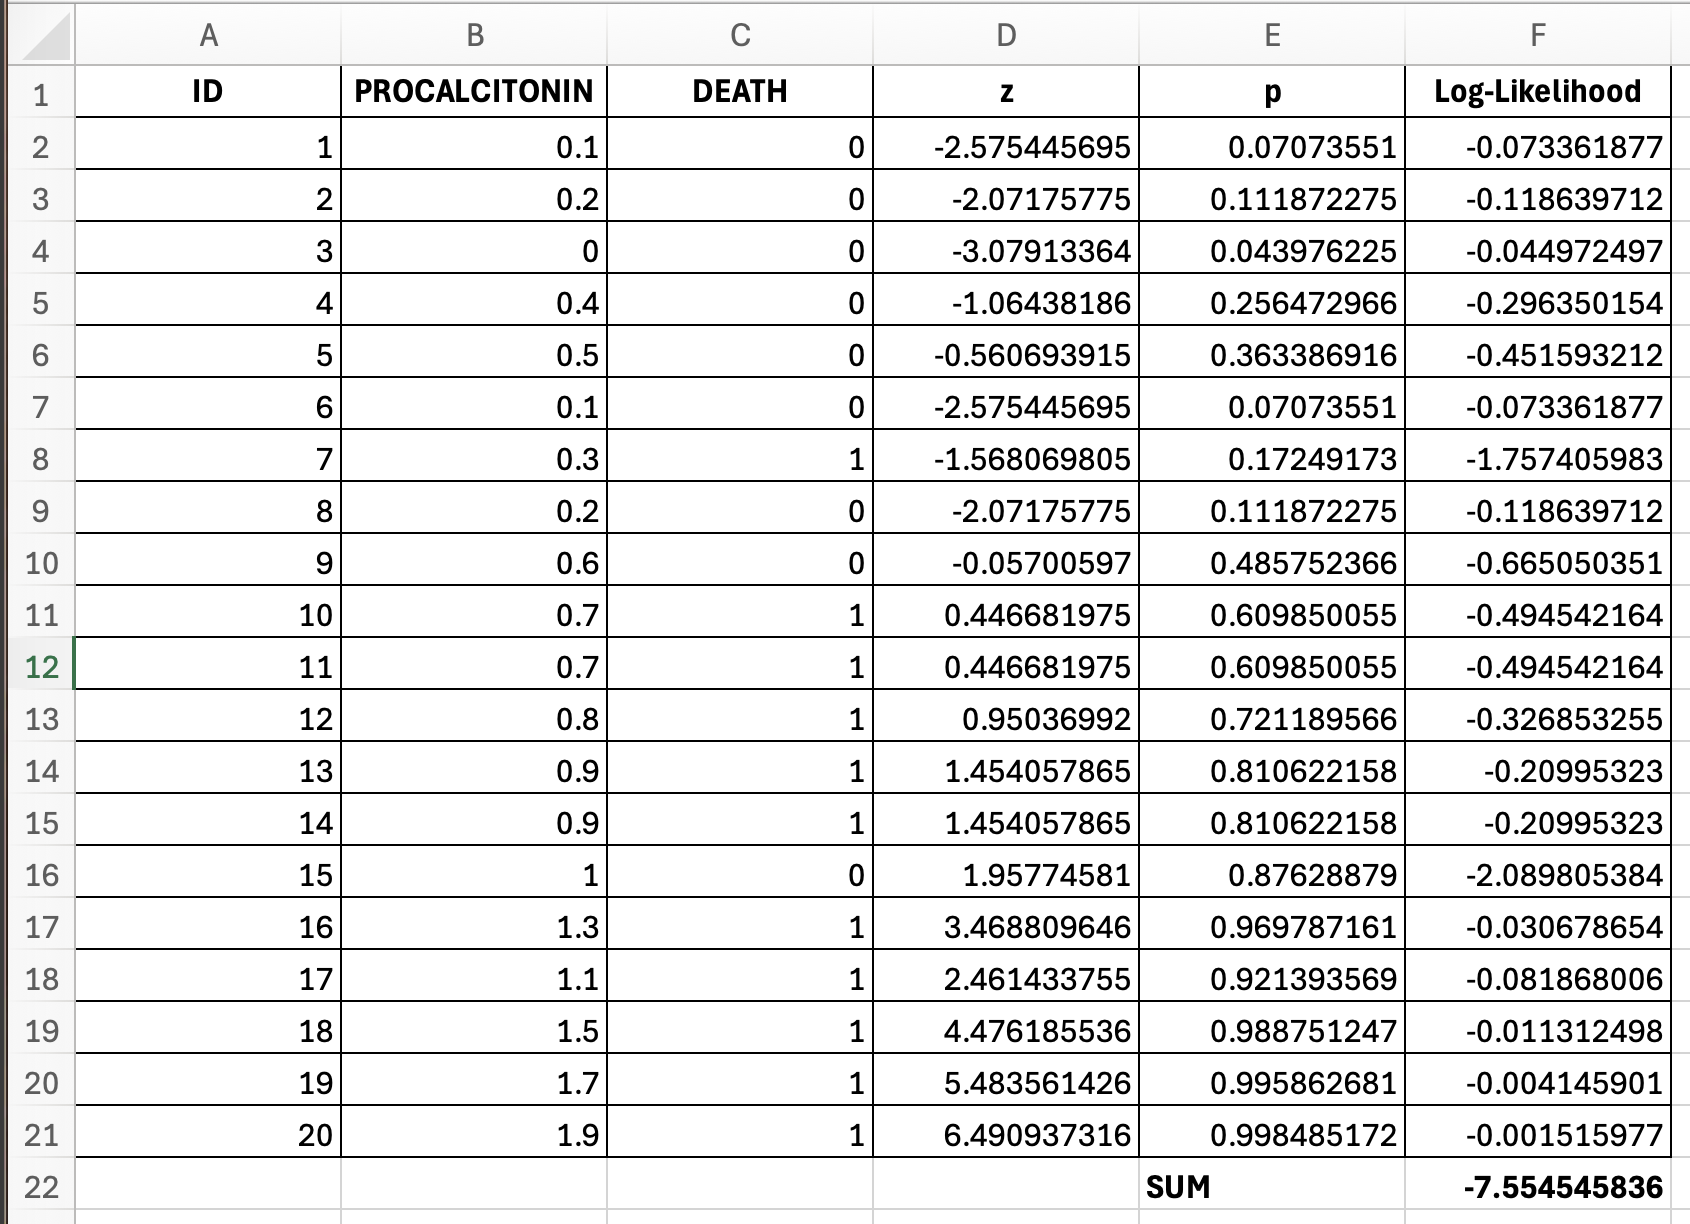
\includegraphics[width=1\textwidth]{LAB04/pics/Excel_calc.png}
    \caption{Tính toán các giá trị $z$, $p$ và Log-Likelihood}
    \label{fig:calc}
\end{figure}

\item Tối ưu bằng Solver

Thiết lập Solver (Hình \ref{fig:solver}):

\begin{itemize}
\item Objective: Maximize tổng Log-Likelihood
\item Variable Cells: $\beta_0, \beta_1$
\item Method: GRG Nonlinear
\end{itemize}

\begin{figure}[!htp]
    \centering
    
\includegraphics[width=0.5\textwidth]{LAB04/pics/Excel_solver.png}
    \caption{Thiết lập Solver để tối ưu tham số}
    \label{fig:solver}
\end{figure}

\item \textbf{Kết quả}

Sau khi tối ưu:

\[
\beta_0 = -3.079,\quad \beta_1 = 5.037
\]

\begin{figure}[!htp]
    \centering
    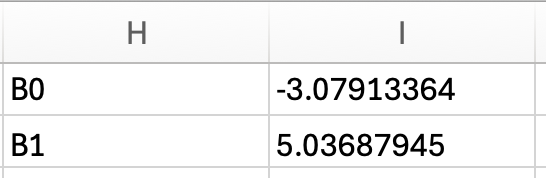
\includegraphics[width=0.4\textwidth]{LAB04/pics/Excel_result.png}
    \caption{Kết quả ước lượng tham số}
    \label{fig:result}
\end{figure}

\end{enumerate}

\subsection{Kết quả mô hình}

Phương trình hồi quy logistic:
\[
p = \frac{1}{1 + e^{-(-3.079 + 5.037X)}}
\]
Dạng logit:
\[
\log\left(\frac{p}{1-p}\right) = -3.079 + 5.037X
\]

% \newpage
\section{Thực hiện Logistic Regression bằng R}
\subsection{Các bước thực hiện}

\begin{enumerate}

\item Nhập dữ liệu vào R

Sử dụng file \texttt{Death\_Probability.csv}:
\begin{verbatim}
data <- read.csv("Death_Probability.csv")
head(data)
\end{verbatim}

\begin{figure}[!htp]
    \centering
    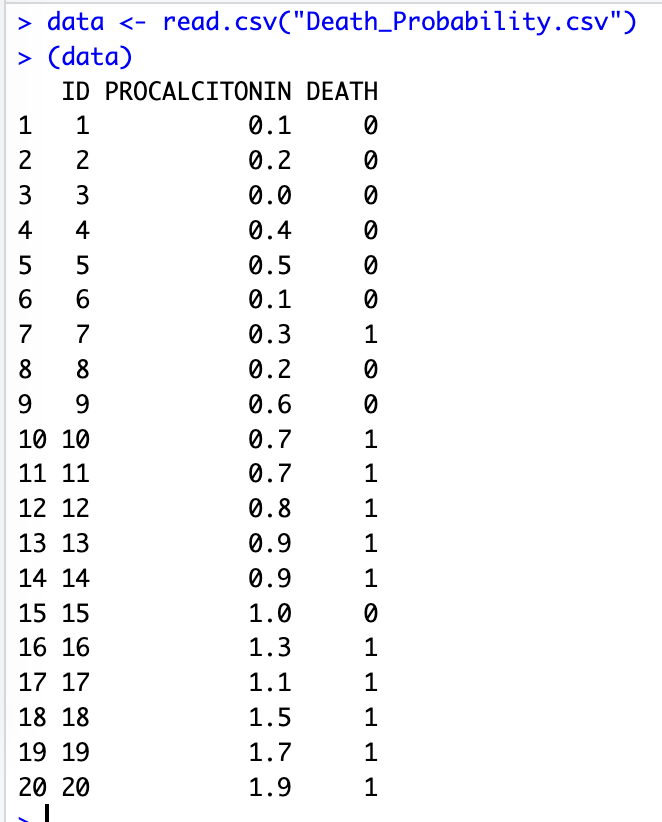
\includegraphics[width=0.6\textwidth]{LAB04/pics/R_data.png}
    \caption{Dữ liệu đầu vào trong R}
    \label{fig:rdata}
\end{figure}

\item Xây dựng mô hình Logistic Regression
\begin{verbatim}
model <- glm(DEATH ~ PROCALCITONIN,
             data = data,
             family = binomial)

summary(model)
\end{verbatim}

\item Kết quả từ output của R:

\[
\beta_0 = -3.079,\quad \beta_1 = 5.037
\]

\begin{figure}[!htp]
    \centering
    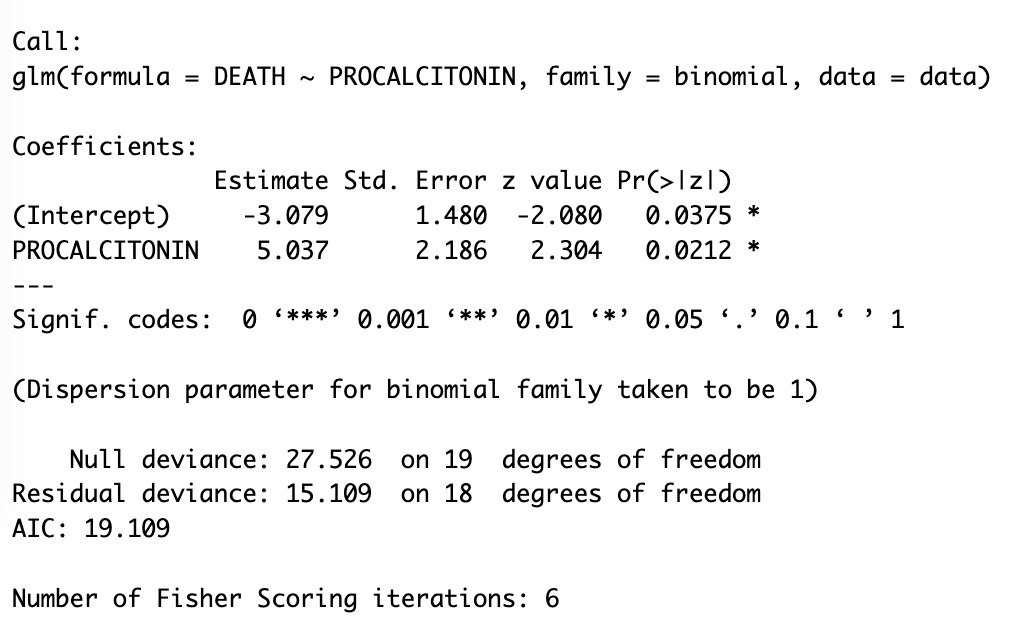
\includegraphics[width=1\textwidth]{LAB04/pics/R_result.png}
    \caption{Kết quả hồi quy logistic trong R}
    \label{fig:rresult}
\end{figure}

\end{enumerate}

\newpage
\section{Thực hiện Logistic Regression bằng SPSS}

\subsection{Các bước thực hiện}

\begin{enumerate}

\item Nhập dữ liệu

Mở phần mềm SPSS và import file \texttt{Death\_Probability.csv}. 
Dữ liệu gồm các biến:

\begin{itemize}
\item ID: mã bệnh nhân
\item PROCALCITONIN: biến độc lập (X)
\item DEATH: biến phụ thuộc (Y)
\end{itemize}

\begin{figure}[!htp]
    \centering
    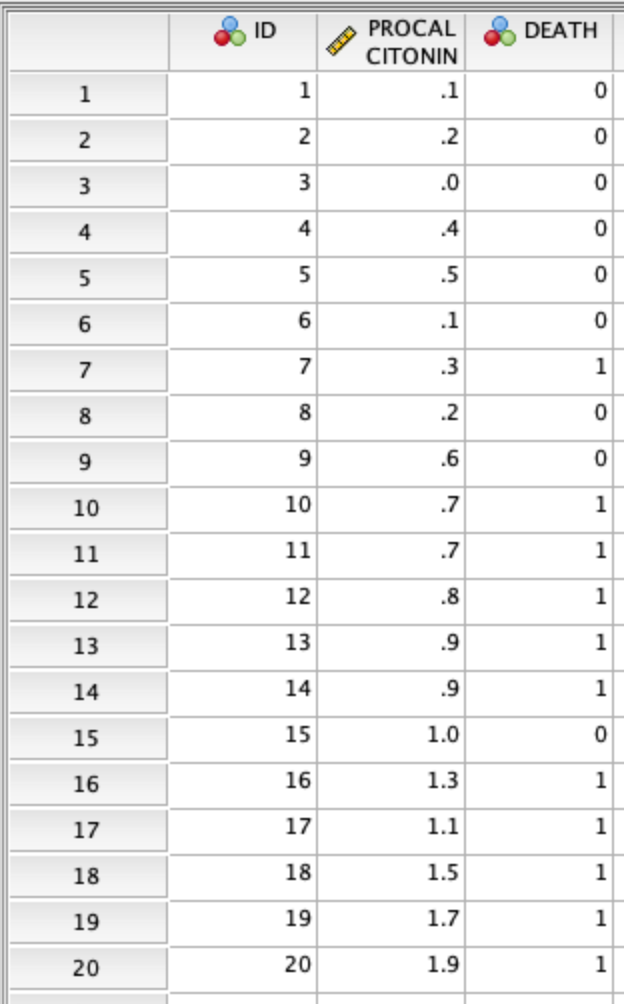
\includegraphics[width=0.6\textwidth]{LAB04/pics/SPSS_data.png}
    \caption{Dữ liệu đầu vào trong SPSS}
    \label{fig:spss_data}
\end{figure}

\item Thiết lập mô hình Logistic Regression

Thực hiện theo các bước:
\begin{itemize}
\item Chọn \textbf{Analyze → Regression → Binary Logistic}
\item Chọn biến \textbf{DEATH} vào ô Dependent
\item Chọn biến \textbf{PROCALCITONIN} vào ô Covariates
\item Nhấn \textbf{Options} và chọn:
\begin{itemize}
\item Hosmer-Lemeshow goodness-of-fit
\item CI for Exp(B) = 95\%
\end{itemize}
\item Nhấn \textbf{OK} để chạy mô hình
\end{itemize}

\begin{figure}[!htp]
    \centering
    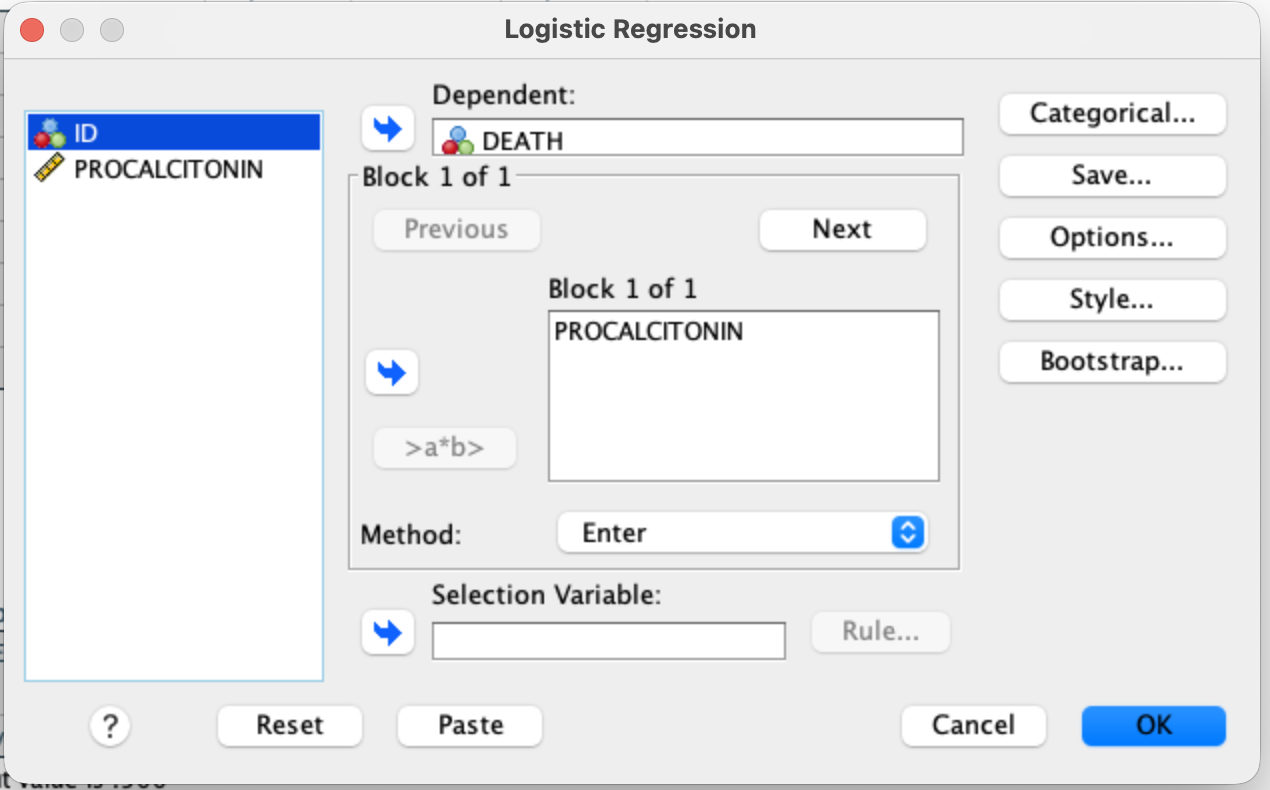
\includegraphics[width=0.8\textwidth]{LAB04/pics/SPSS_setup.png}
    \caption{Thiết lập mô hình Logistic Regression trong SPSS}
    \label{fig:spss_setup}
\end{figure}
\item Xuất kết quả

Sau khi chạy mô hình, SPSS cung cấp các bảng kết quả, trong đó bảng \textbf{Variables in the Equation} được sử dụng để xác định các hệ số hồi quy.

\begin{figure}[!htp]
    \centering
    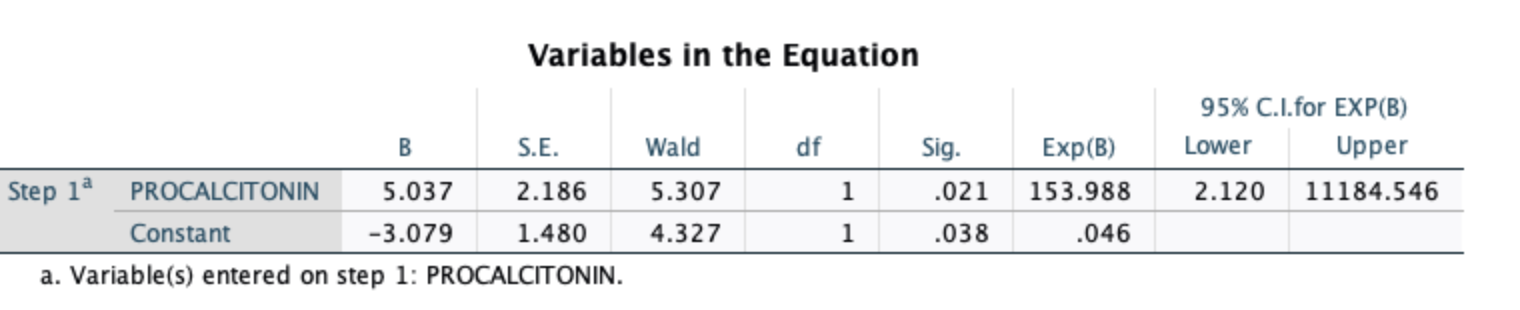
\includegraphics[width=1\textwidth]{LAB04/pics/SPSS_result.png}
    \caption{Kết quả hồi quy logistic trong SPSS}
    \label{fig:spss_result}
\end{figure}

\end{enumerate}

\subsection{Kết quả mô hình}

Từ kết quả SPSS:

\[
\beta_0 = -3.079,\quad \beta_1 = 5.037
\]

Phương trình hồi quy logistic:

\[
\log\left(\frac{p}{1-p}\right) = -3.079 + 5.037X
\]

\textbf{Nhận xét:}

\begin{itemize}
\item Hệ số $\beta_1 > 0$ cho thấy mối quan hệ cùng chiều giữa PROCALCITONIN và xác suất tử vong
\item Giá trị Sig = 0.021 < 0.05, biến PROCALCITONIN có ý nghĩa thống kê
\end{itemize}

\newpage
\section{Thực hiện Logistic Regression bằng Python}

\subsection{Các bước thực hiện}

\begin{enumerate}

\item Nhập thư viện và dữ liệu

Sử dụng thư viện \texttt{pandas} và \texttt{statsmodels} để xử lý dữ liệu và xây dựng mô hình:

\begin{verbatim}
import pandas as pd
import statsmodels.api as sm

data = pd.read_csv("Death_Probability.csv")
data.head()
\end{verbatim}

\begin{figure}[!htp]
    \centering
    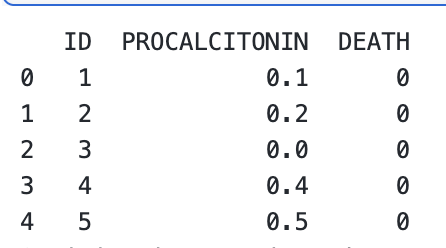
\includegraphics[width=0.6\textwidth]{LAB04/pics/Python_data.png}
    \caption{Dữ liệu đầu vào trong Python}
    \label{fig:pydata}
\end{figure}

\item Chuẩn bị dữ liệu

Xác định biến độc lập và biến phụ thuộc, đồng thời thêm hệ số chặn:

\begin{verbatim}
X = data["PROCALCITONIN"]
Y = data["DEATH"]

X = sm.add_constant(X)
\end{verbatim}

\item Xây dựng mô hình Logistic Regression

\begin{verbatim}
model = sm.Logit(Y, X)
result = model.fit()

print(result.summary())
\end{verbatim}

\item Xuất kết quả

Lấy các hệ số hồi quy từ mô hình:

\begin{verbatim}
result.params
\end{verbatim}

\begin{figure}[!htp]
    \centering
    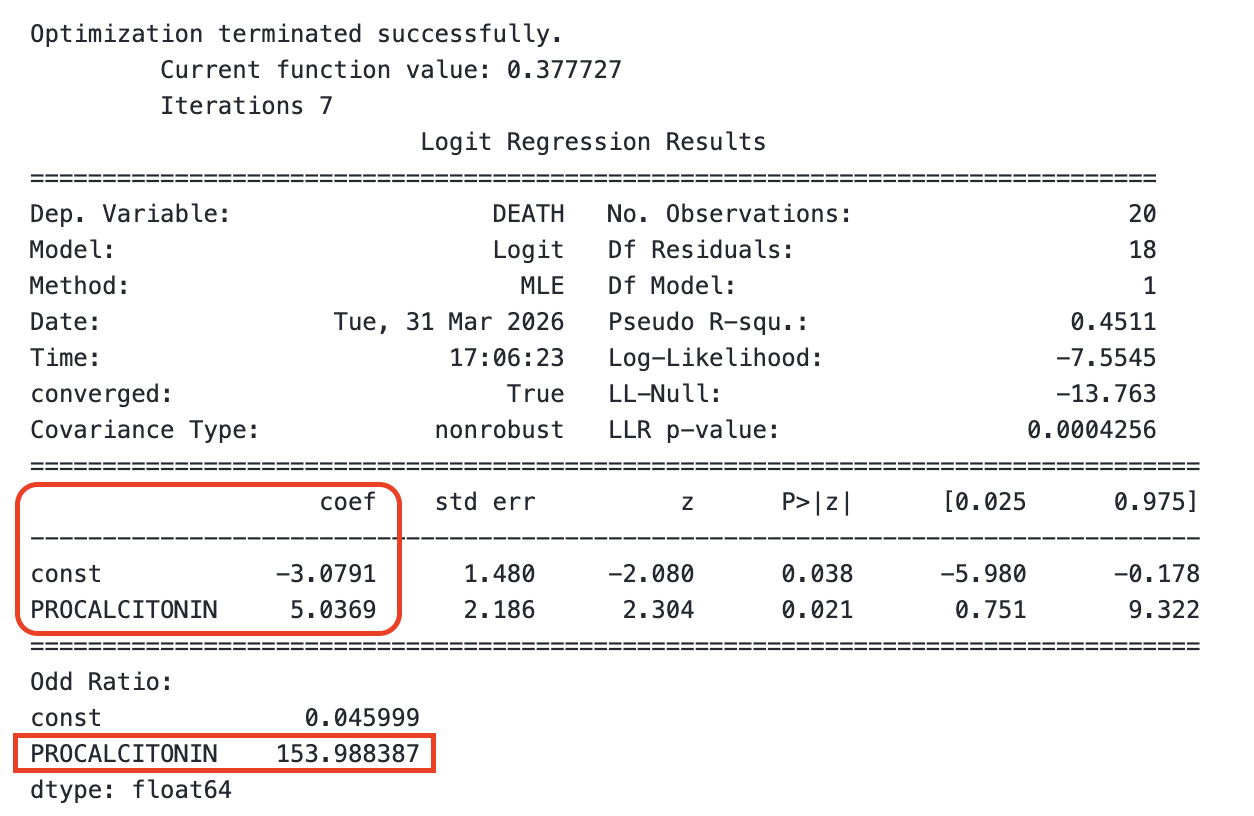
\includegraphics[width=01\textwidth]{LAB04/pics/Python_result.png}
    \caption{Kết quả hồi quy logistic trong Python}
    \label{fig:pyresult}
\end{figure}

\end{enumerate}

\subsection{Kết quả mô hình}

Từ kết quả Python:

\[
\beta_0 = -3.079,\quad \beta_1 = 5.037
\]

Phương trình hồi quy logistic:

\[
\log\left(\frac{p}{1-p}\right) = -3.079 + 5.037X
\]

\textbf{Nhận xét:}

\begin{itemize}
\item Hệ số $\beta_1 > 0$ cho thấy mối quan hệ cùng chiều giữa PROCALCITONIN và xác suất tử vong
\item Giá trị p-value < 0.05 cho thấy biến PROCALCITONIN có ý nghĩa thống kê trong mô hình
\end{itemize}

\section{Kết quả mô hình từ các công cụ đã sử dụng}

\subsection{Phương trình hồi quy logistic:}

\[
p = \frac{1}{1 + e^{-(-3.079 + 5.037X)}}
\]

Dạng logit:

\[
\log\left(\frac{p}{1-p}\right) = -3.079 + 5.037X
\]

\textbf{Diễn giải hệ số:}

\begin{itemize}
\item $\beta_1 > 0$: mối quan hệ cùng chiều
\item Khi PROCALCITONIN tăng, xác suất tử vong tăng
\item p-value của biến PROCALCITONIN = 0.0212 < 0.05 $\Rightarrow$ có ý nghĩa thống kê
\end{itemize}

\subsection{Phân tích Odds}

Odds được định nghĩa:

\[
Odds = \frac{p}{1-p} = e^{\beta_0 + \beta_1 X}
\]

\subsubsection{Trường hợp $X = 0$ (PROCALCITONIN = 0)}

\[
z = -3.079
\]

\[
p = \frac{1}{1 + e^{3.079}} \approx 0.044
\]

\[
Odds_0 = \frac{0.044}{0.956} \approx 0.046
\]

Trong trường hợp này, xác suất tử vong của bệnh nhân khoảng 4.4%, cho thấy nguy
cơ tử vong rất thấp. Bệnh nhân có tiên lượng tốt và khả năng sống cao
\subsubsection{Trường hợp $X = 1$ (PROCALCITONIN = 1)}

\[
z = -3.079 + 5.037 = 1.958
\]

\[
p = \frac{1}{1 + e^{-1.958}} \approx 0.876
\]

\[
Odds_1 = \frac{0.876}{0.124} \approx 7.085
\]

Trong trường hợp này, xác suất tử vong của bệnh nhân khoảng 87.6%, cho thấy nguy cơ tử vong rất cao. Bệnh nhân ở trạng thái nguy hiểm và cần được theo dõi, can thiệp y tế kịp thời.

\subsubsection{Tỷ số Odds (Odds Ratio)}

\[
OR = \frac{Odds_1}{Odds_0} \approx 154
\]

Ngoài ra:

\[
OR = e^{\beta_1} = e^{5.037} \approx 154
\]


\subsection{Diễn giải, so sánh và tiên lượng khả năng tử vong}

Khi PROCALCITONIN tăng 1 đơn vị, odds tử vong tăng khoảng 154 lần. 
Điều này cho thấy PROCALCITONIN là một biến có ảnh hưởng rất mạnh đến xác suất tử vong và có thể sử dụng trong dự báo lâm sàng.

